\documentclass{article}
\usepackage[utf8]{inputenc}
\usepackage{graphicx}
\usepackage[margin=1in]{geometry}
\usepackage{float}
\usepackage{epstopdf}
\usepackage{wrapfig}

\title{Circuits Lab 7}
\author{Dan Kearney and Theo Thompson}
\date{April 11, 2013}

\begin{document}
\maketitle
In this lab, we studied the MOS differential pair. This circuit is useful because it has a large response for small differences between its input voltages, which is why it is used in op-amps.
\section*{Experiment 1: Differential Pair Current–Voltage Characteristics}
In this experiment, we examined the current-voltage characteristics for different values of the common-mode input, while sweepingthe differential-mode input. We also took measurements for two different levels of bias current, one where the bias transistor is below saturation and one where it is above. The schematic we used to construct this circuit is shown in figure \ref{schem}. 
\begin{figure}[H]
\centering
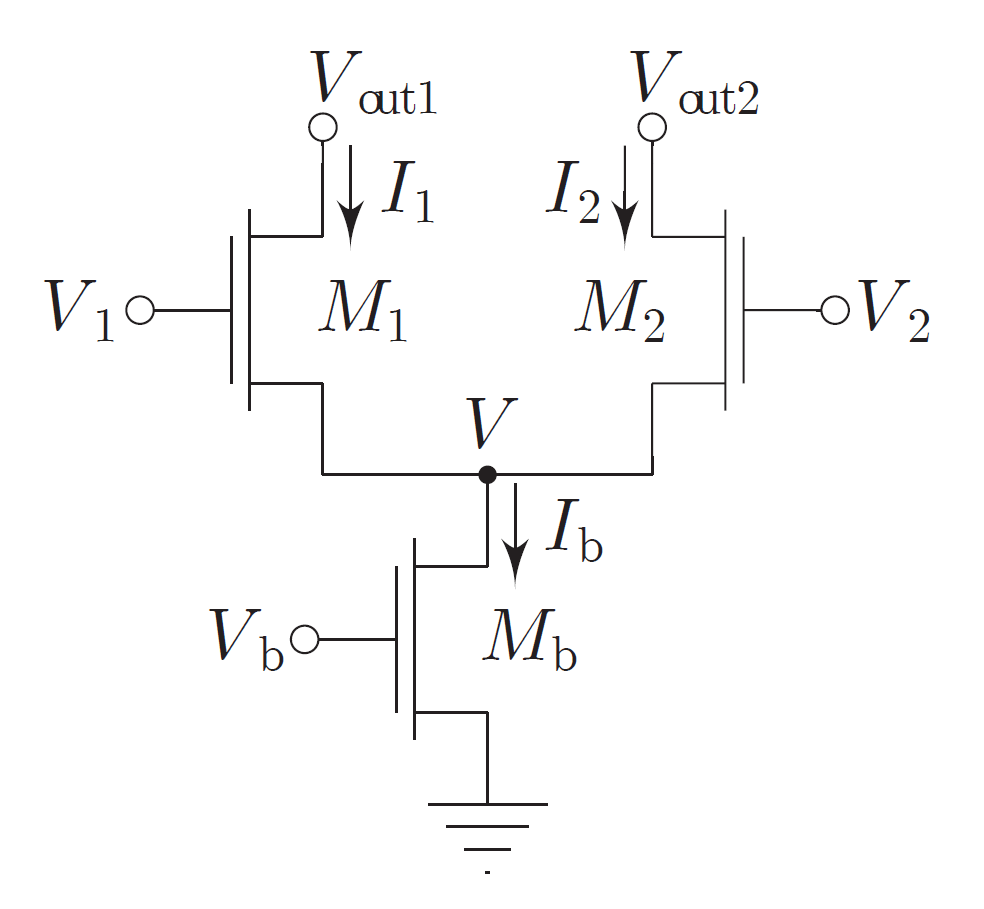
\includegraphics[scale=.3]{diffSchem.png}
\label{schem}
\caption{The nMOS differential pair}
\end{figure}

\subsubsection*{Weakly Inverted Bias Transistor}
To examine the current-voltage characteristic for low bias current levels, we set $V_b$ below threshold but kept the bias transistor saturated. We used a value of .55 V, knowing that the bias transistor's threshold voltage is around .6 V.  This set the bias current low (the single microamp range), which resulted in low values for $I_1$ and $I_2$ (we know this from KCL: $I_1+I_2=I_b$). We swept the difference between $V_1$ and $V_2$ by sweeping $V_1$ from $.3V$ below $V_2$ to $.3V$ above $V_2$. We measured the output currents $I_1$ and $I_2$ and calculated their sum and difference. We did this for several values of the common mode input voltage ($2V,3V,4V$). As we alluded to in the prelab, we chose those three voltages such that the common node voltage always allowed the bias transistor to remain in saturation.  The plot is shown in figure \ref{weak}.\\

Theoretically, we know that the sum of $I_1$ and $I_2$ should be constant because $I_b$ is set by the bias transistor. This is confirmed in the plot. We also see that when $V_1$ is more than a tenth of a volt above $V_2$, $I_1 \approx I_b$ and $I_2 \approx 0$. Similarly, when $V_1$ is more than a tenth of a volt below $V_2$, $I_2 \approx I_b$ and $I_1 \approx 0$. We showed this in the prelab assignment. Our experimental data confirms this relationship. We also see that when $V_1=V_2$, $I_1=I_2$.\\

We know that since the bias transistor is in weak inversion, the other two transistors must always be in weak inversion. Since $M_1$ and $M_2$ have at most the same amount of channel current as $M_b$, we can say that $M_1$ and $M_2$ are at the same inversion level as $M_b$. In weak inversion, the current is exponentially related to the gate-source voltage. This is why any difference between $V_1$ and $V_2$ causes a rapid change in output currents: they are exponentially related. \\

Changing the common mode input voltage does not have a significant effect on the output currents. The difference between $V_1$ and $V_2$ is what changes the output.\\

To calculate the incremental differential mode transconductance gain, we fit a line to the difference between $I_1$ and $I_2$ for small values of $V_{dm}$ and extracted the slope. The results are shown in the table below. Note that $V_{CM}$ does not significantly change these values - the transconductance gain is not affected by the average input voltage!
\\
\begin{center}
\begin{tabular} {|c|c|}
\hline
$V{CM}$ (Volts) & $G_{DM}$ (Mhos) \\ 
\hline
2V & $1.76 *10^{-5}$ \\
3V & $1.78 *10^{-5}$ \\
4V & $1.91 *10^{-5}$ \\
\hline
\end{tabular}

\end{center}

\begin{figure}[H]
\centering
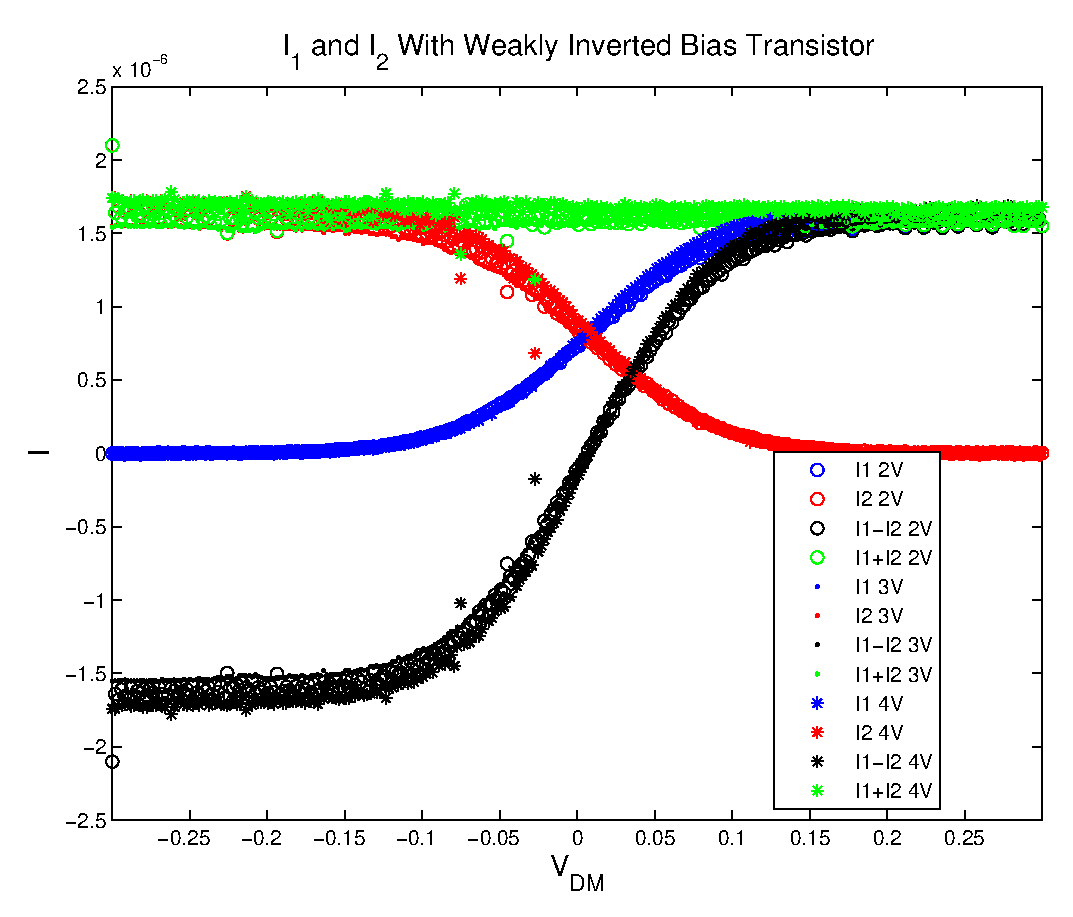
\includegraphics[scale=.8]{currents_weak.eps}
\caption{Our current measurements when the bias transistor gate voltage below threshold.}
\label{weak}
\end{figure}

Next we measured the common node voltage, $V$. From the prelab, we know that: \[V= \kappa (max(V_1,V_2)-V_b)\]
Figure \ref{weakV} shows our experimental findings. At the beginning of our sweep, $V_1<V_2$. Therefore $V=\kappa(V_2-V_b)$. Since we held $V_2$ constant, we know that $V$ should also be constant. As we sweep $V_1$ higher than $V_2$, $V=\kappa(V_1-V_b)$. The common node voltage then becomes linear because $V_1$ is steadily increasing from the sweep. In between, there is a small nonlinear transition region, but because the current response is exponential, this region is small.

\begin{figure}[H]
\centering
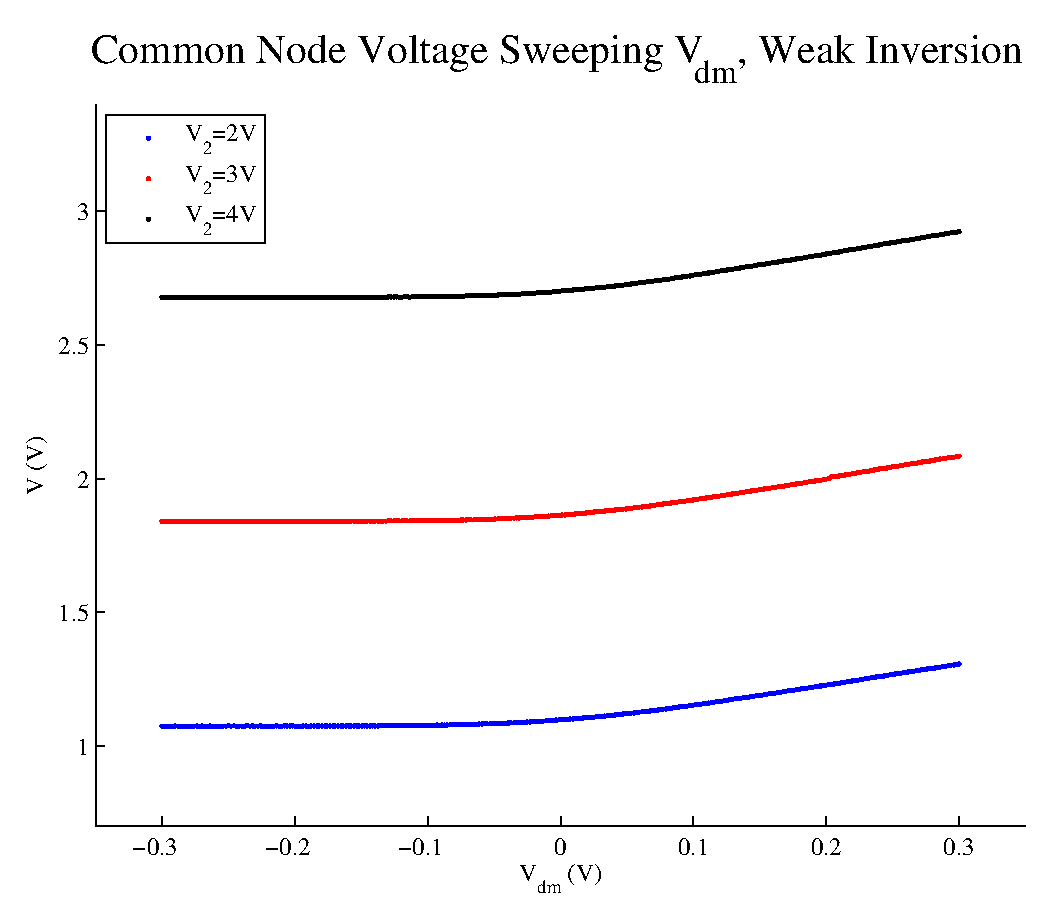
\includegraphics[scale=.7]{plot_weak_v.eps}
\caption{The common node voltage in response to a sweep of $V_1$}
\label{weakV}
\end{figure}

\subsubsection*{Strongly Inverted Bias Transistor}

We then put $V_b$ above threshold so that the bias transistor was in strong inversion. We took the same current measurements as before, shown in figure \ref{strong}. The output behavior is very similar to when the bias transistor was in weak inversion. The major difference is that the output currents are less sensitive to the differential mode current. In weak inversion, we saw that they were exponentially related. Since all the transistors are in strong inversion (we showed that they must all be the same earlier), the channel current is now \emph{quadratically} related to the gate-source voltage. Now, there needs to be a difference of about $.4V$ for $I_1$ or $I_2$ to equal the bias current. \\

\begin{figure}[H]
\centering
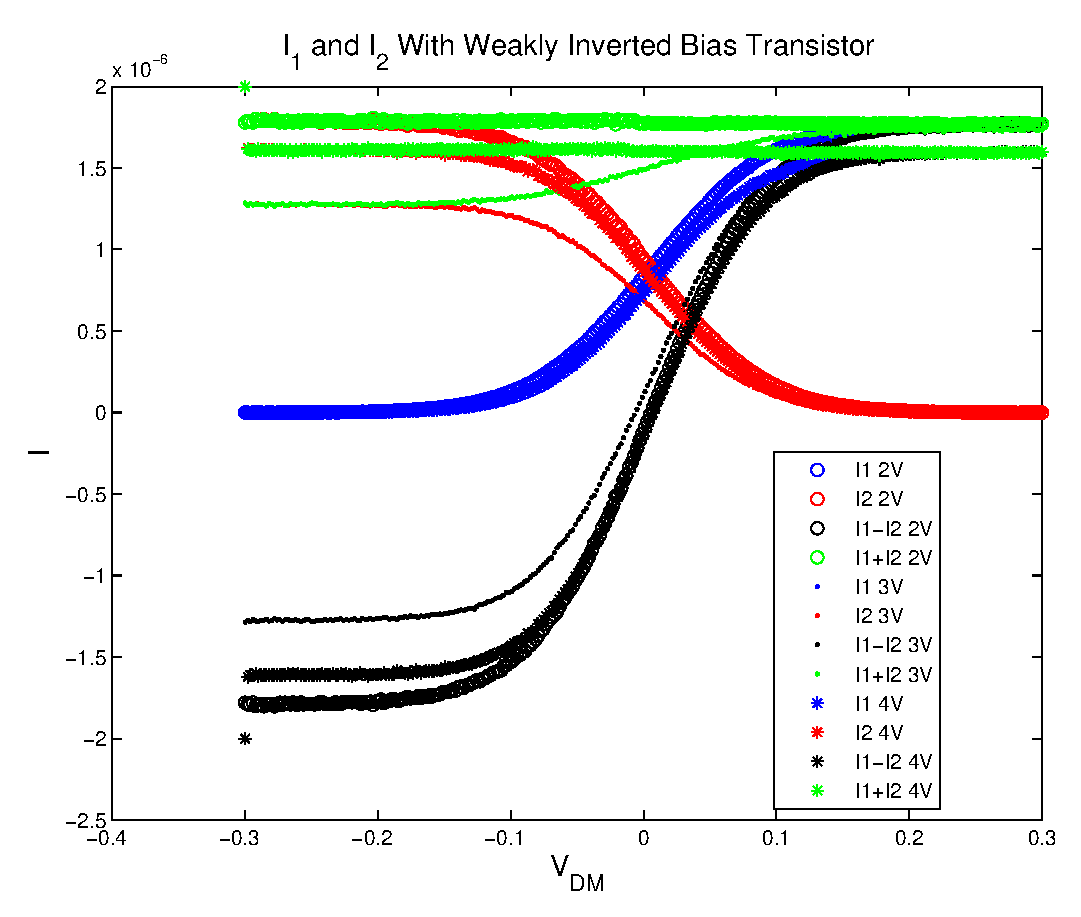
\includegraphics[scale=.8]{currents_strong.eps}
\caption{Our current measurements when the bias transistor gate voltage above threshold.}
\label{strong}
\end{figure}

We calculated the incremental differential mode transconductance gain when the bias transistor was in strong inversion. The results are shown in the table below. Note that $V_{CM}$ does not significantly change these values.

\begin{center}
\begin{tabular} {|c|c|}
\hline
$V{CM}$ (Volts) & $G_{DM}$ (Mhos) \\ 
\hline
2  & $1.77 *10^{-4}$ \\
3 & $1.83 *10^{-4}$ \\
4 & $1.87 *10^{-4}$ \\
\hline
\end{tabular}
\end{center}

We also examined the common node voltage. The result is very similar to the weak inversion case (\ref{strongV}).

\begin{figure}[H]
\centering
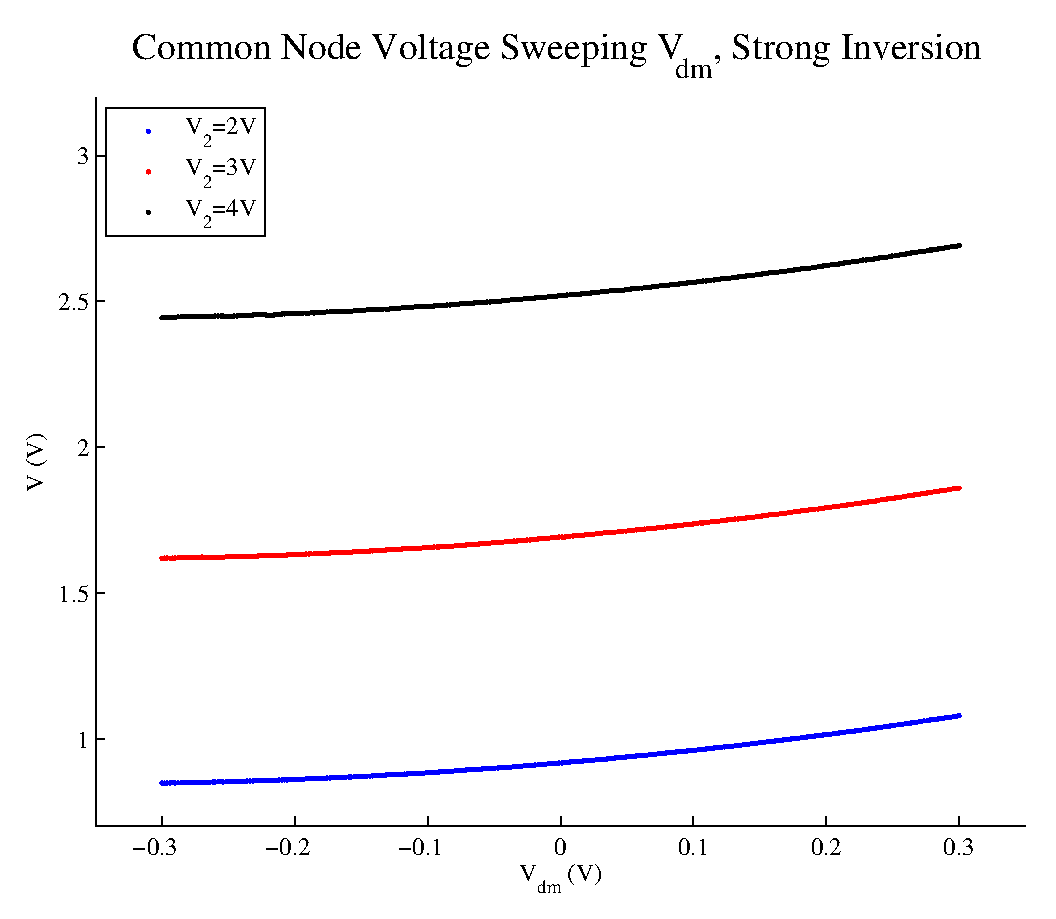
\includegraphics[scale=.7]{plot_strong_v.eps}
\caption{The common node voltage in response to a sweep of $V_1$}
\label{strongV}
\end{figure}

For negative $V_{dm}$, the common node voltage holds steady at $V_2$.  For positive $V_{dm}$, the voltage slowly transitions to a linear function of $V_{1}$.  The transition region for the strongly inverted differential pair is significantly slower than that of the weakly inverted pair.  That is because the current response of the circuit is quadratic in strong inversion, so it takes longer for either transistor to dominate the other than in weak inversion, which is governed by an exponential.  This is because exponentials grow faster than quadratics.

\section*{Conclusion}

The differential pair is an interesting circuit because the current difference responds much more quickly to change in input in weak inversion than in strong inversion - which is counter-intuitive.


\end{document}